
\section{Tesztelés}

\subsection{A teszteléshez használt eszközök}
\label{sec:tesztelesi_eszkozok}

A teszteléshez az Ericsson SDS által nyújtott eszközöket használtam. A kliens alkalmazás tesztelését két notebook felhasználásával végeztem, mivel egy operációs rendszeren csak egy felhasználói profillal rendelkező ICP futtatható. A két kliens Alice és Bob felhasználónévvel, illetve a nevekhez illeszkedő SIP URI-val rendelkeznek (például: sip:alice@ericsson.com). A kliens és a szerver közötti kommunikációs folyamatok teszteléséhez, az üzenetek megjelenítéséhez az SDS-ben megtalálható Visual Traffic Flow-t használtam. 

\subsection{Az teljes üzenetküldés kommunikációs folyamatának tesztelése}
\label{sec:teszteles_teljes_kuldes}

Amikor egy felhasználó multimédia üzenetet küld egy kiválasztott csoportnak, a multimédia üzenet tartalmát MSRP kapcsolaton el kell küldenie a szerver oldalnak. A tartalom átvitelének folyamata előtt a kliens és a szerver között fel kell építeni egy MSRP kapcsolatot. Miután a kapcsolat sikeresen kiépült, a multimédia üzenet tartalma átvitelre kerül, majd az átvitel végén a kliens oldal egy SIP MESSAGE kérésben elküldi az üzenet egyéb adatait (például a címzetteket, az üzenet tárgyát, stb). Az üzenetküldés folyamatának zárásaként bontani kell az MSRP kapcsolatot. \Aref{fig:teszt-vtf-kuldes-01}.~ábrán látható kommunikációs folyamat egy kliens és a szerver közötti multimédia üzenetküldés teljes folyamatát mutatja be. Az ábra VTF segítségével készült. Látható, hogy a kommunikációs folyamat megfelel \aref{sec:kliens_pc}.~pontban felvázolt üzenetküldési folyamatnak (\ref{fig:sending_proc}.~ábra).

\begin{figure}[htb]
\center
\resizebox{14.5cm}{!}{
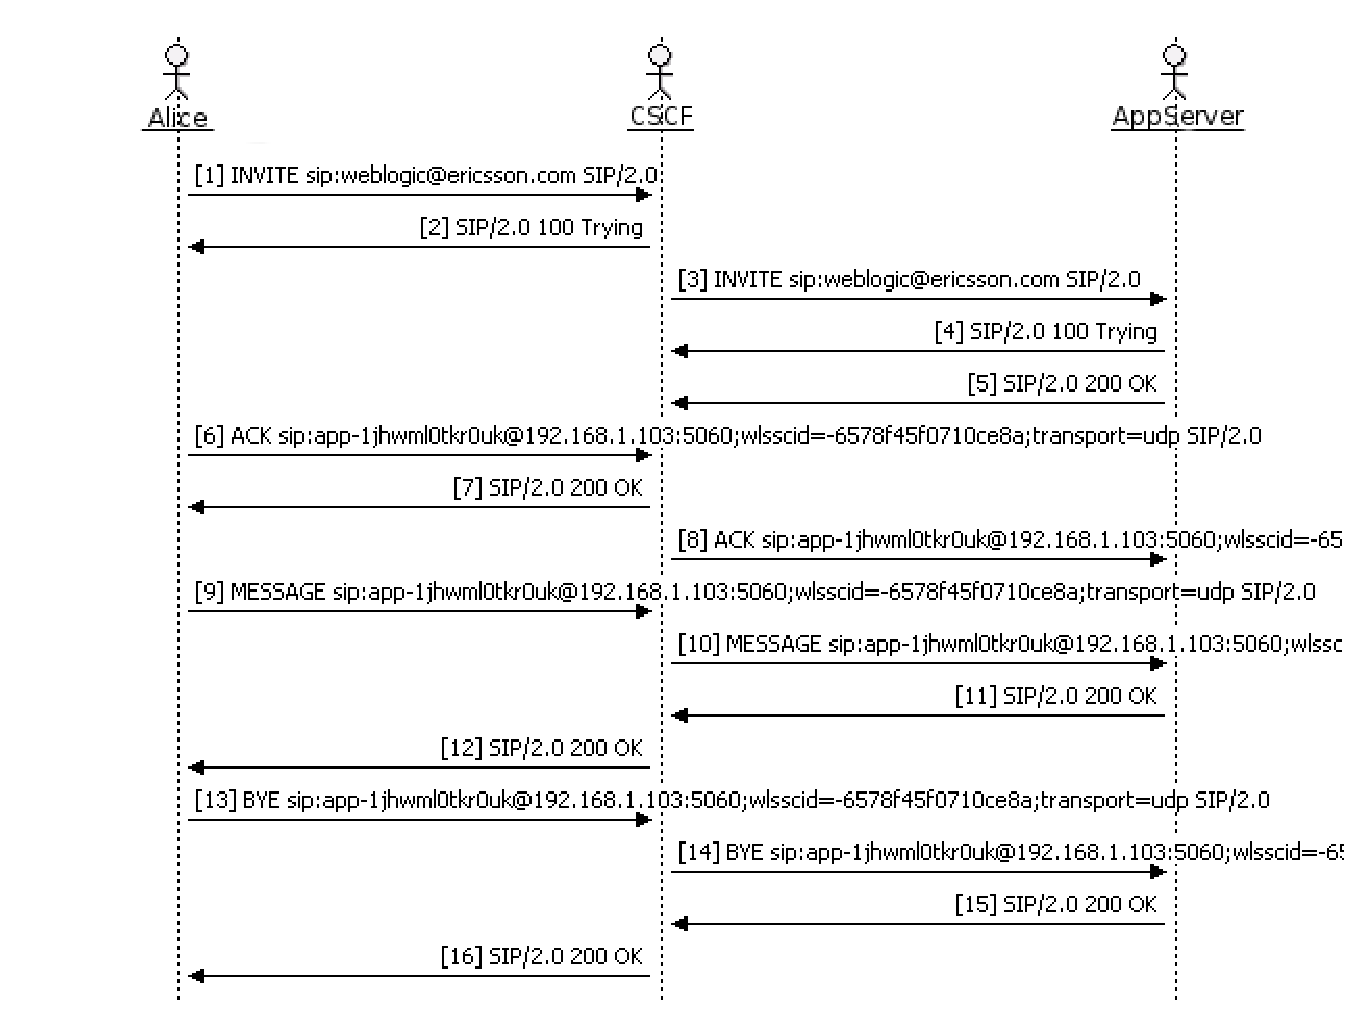
\includegraphics{img/vtf-kuldes-01.eps}}
\caption{Alice üzenetet küld egy csoportnak}
\label{fig:teszt-vtf-kuldes-01}
\end{figure}

\subsection{A késleltetett üzenetkézbesítés tesztelése}
\label{sec:teszteles_kesleltetett_kezbesites}

Abban az esetben, amikor egy felhasználó új üzeneteket kap, miközben ő maga nem elérhető a hálózaton, akkor a szolgáltatásnak kötelessége értesítenie a beérkezett új multimédia üzenetekről a felhasználót, amikor az regisztrál a hálózaton. Az előző, \ref{sec:teszteles_teljes_kuldes}.~pontban leírt üzenetküldés során Alice egy olyan felhasználói csoportnak címezte az üzenetet, amelynek Bob is tagja. Amikor Bob regisztrál a hálózaton, a szerver oldalon futó szolgáltatás értesíti őt Alice (és a többi új) üzenetről. A kommunikációs folyamat \aref{fig:teszt-vtf-ertesites-01}.~ábrán követhető nyomon. Az ábrán jól látható, hogy Bob regisztrációs üzenetének vételekor a szerver értesítő SIP MESSAGE kérést küld Bobnak, amely tartalmazza az új multimédia üzenetek adatait.

\begin{figure}[htb]
\center
\resizebox{14.5cm}{!}{
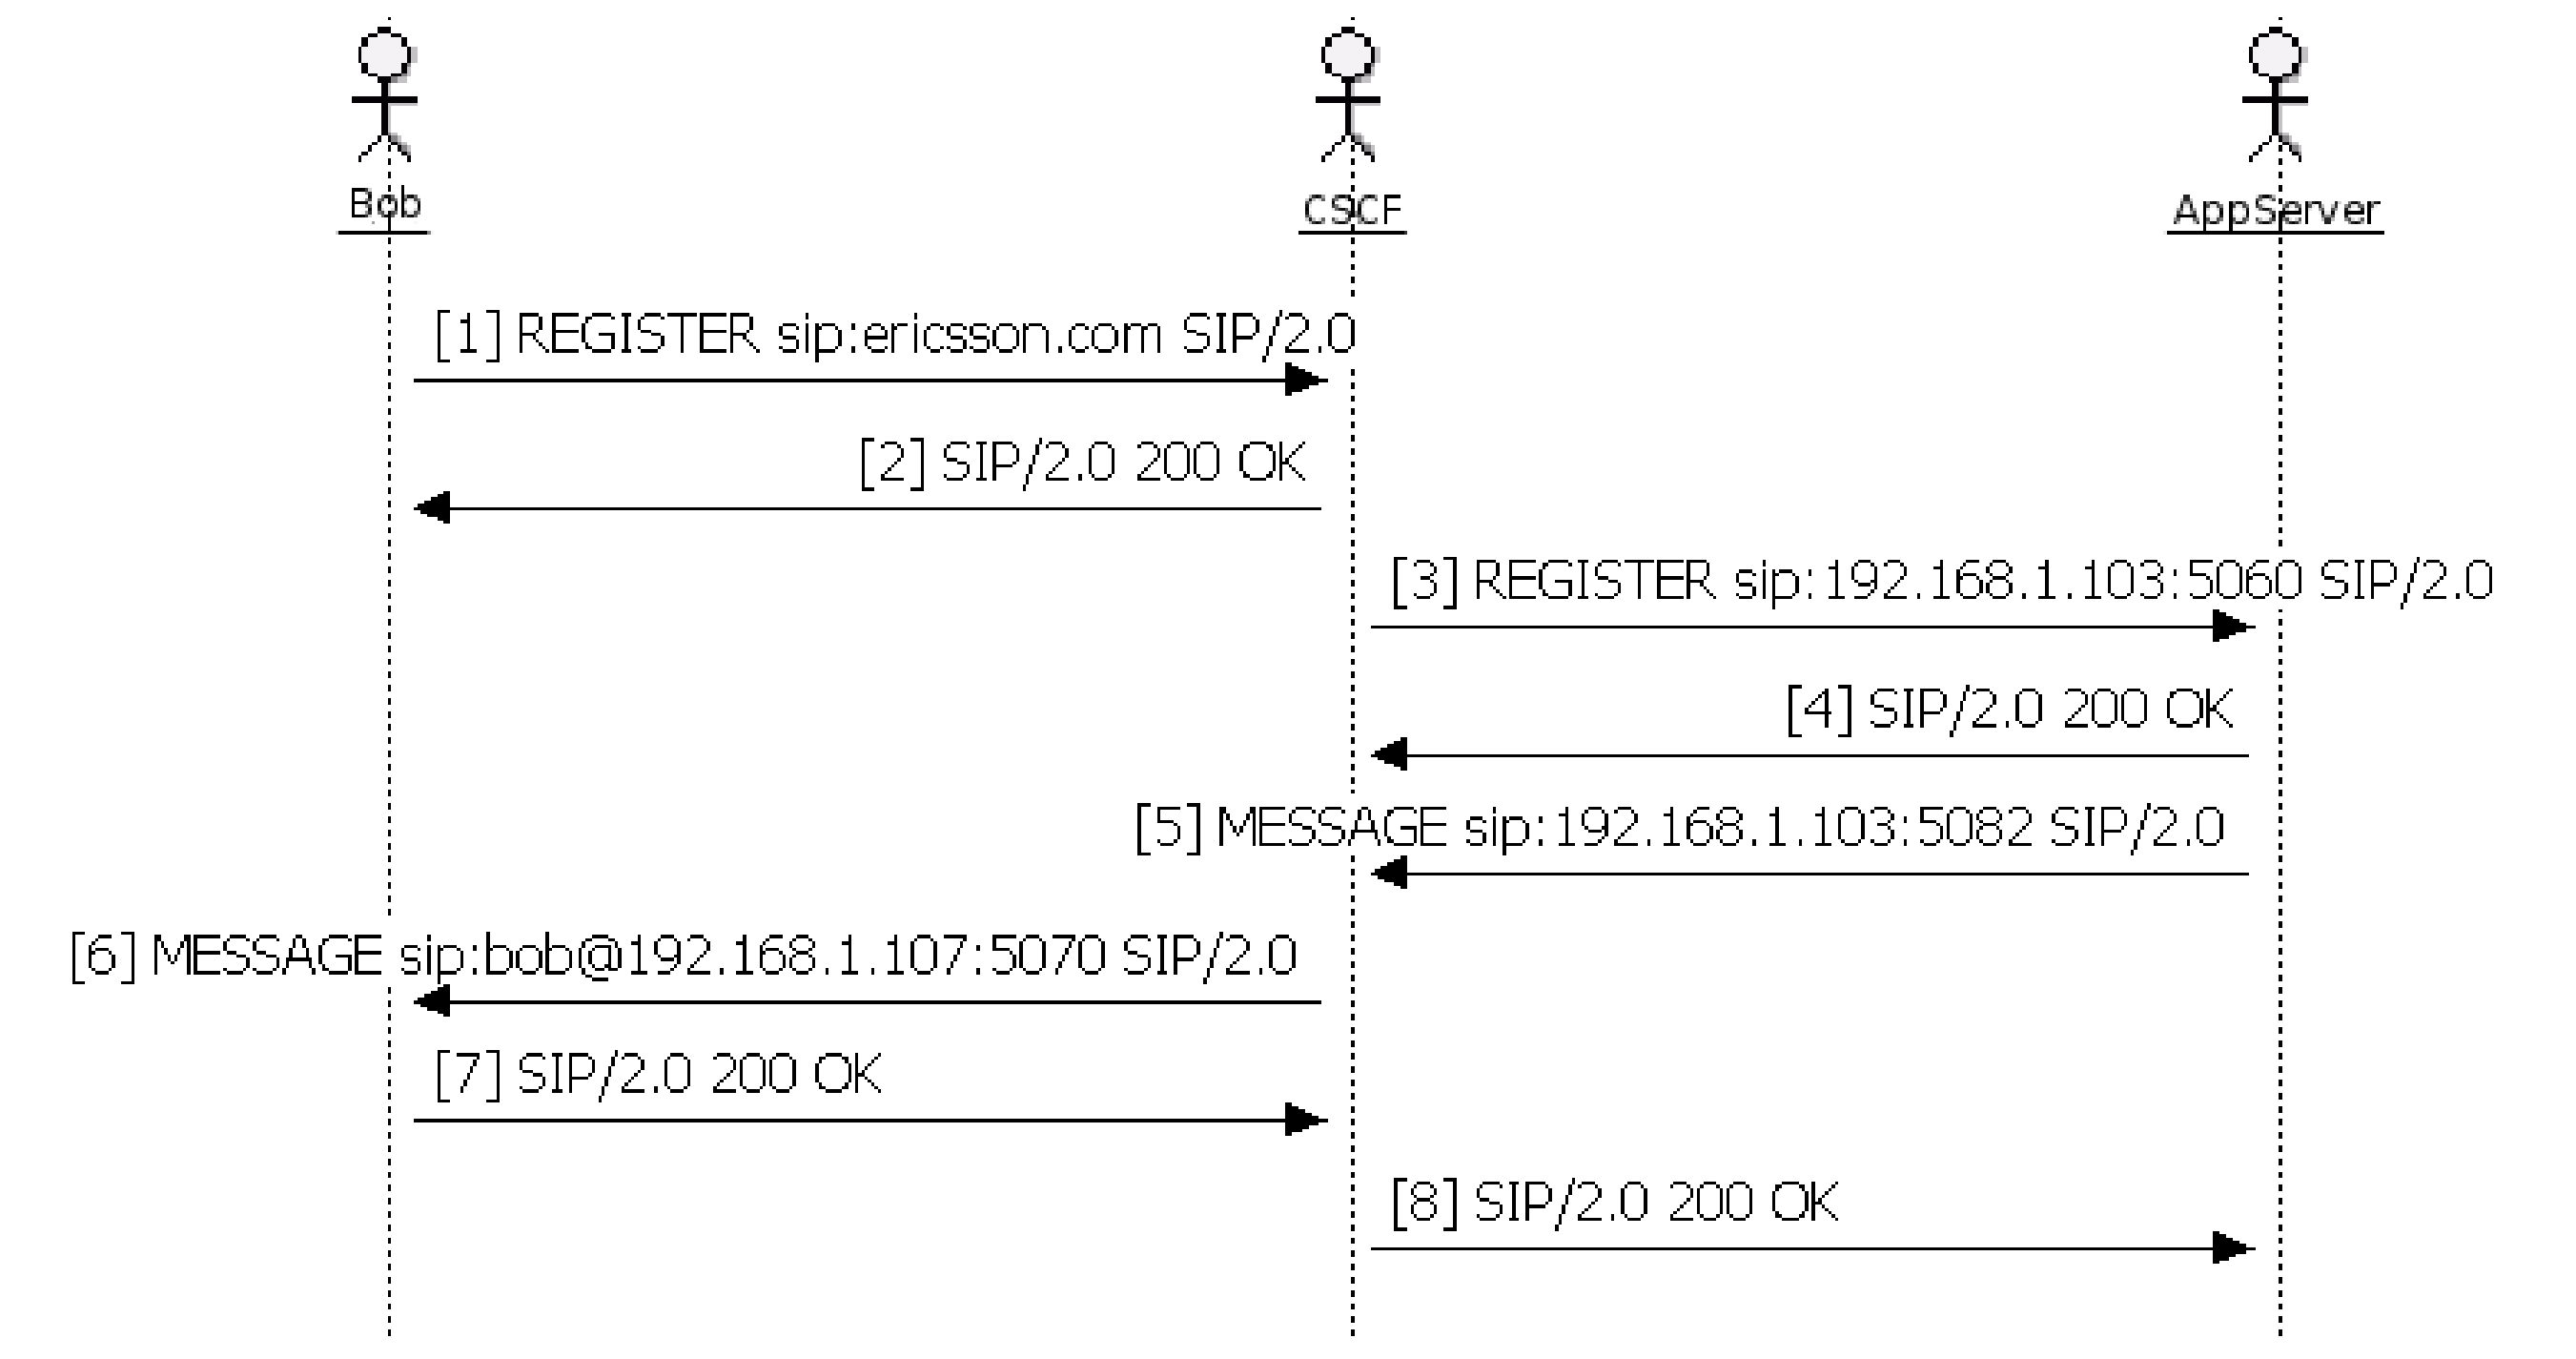
\includegraphics{img/vtf-kuldes-02.eps}}
\caption{A szolgáltatás értesíti Bob-ot az új üzeneteiről}
\label{fig:teszt-vtf-ertesites-01}
\end{figure}

\subsection{A multimédia tartalom letöltésének tesztelése}
\label{sec:teszteles_letoltes}

Bob, miután sikeresen feldolgozta a szervertől kapott értesítő SIP MESSAGE adatait, dönthet úgy, hogy egy adott üzenethez a multimédia tartalmat letölti a szervertől. Az átvitelhez első lépésként fel kell építenie egy MSRP kapcsolatot a szerverrel. Második lépésként Bob egy SIP MESSAGE kérésben jelzi a szervernek, hogy melyik multimédia üzenetek tartalmát szeretné letölteni, majd a kívánt tartalom sikeres átvitele után bontani kell az MSRP kapcsolatot a szerverrel. A tesztelés során a folyamat teljesen megegyezett \aref{fig:teszt-vtf-kuldes-01}.~ábrán felvázolt üzenetküldés folyamatával, csak a 9. üzenetben elküldött XML az üzenet címzettjei, egyéb adatai helyett a letöltési igény adatait tartalmazza.



